\documentclass[12pt,preprint]{aastex}

\usepackage{verbatim}
\usepackage{color}
\usepackage[normalem]{ulem} % for striking out with \sout
\usepackage{amsmath} % for boldsymbol
% A comment block

%\newcommand{\comment}[1]{}

% For color
\newcommand{\mpname}[1]{#1_color.eps}
\newcommand{\clraitoff}{red}
\newcommand{\lumblack}{(black)}
\newcommand{\lumblue}{(blue)}
\newcommand{\lumred}{(red)}
\newcommand{\vdisred}{(red-dashed curve)}
\newcommand{\vdisblue}{(blue-solid curve)}

% For bw
%\newcommand{\mpname}[1]{#1.eps}
%\newcommand{\clraitoff}{}
%\newcommand{\lumblack}{}
%\newcommand{\lumblue}{}
%\newcommand{\lumred}{}
%\newcommand{\vdisred}{(dashed curve)}
%\newcommand{\vdisblue}{(solid curve)}

\newcommand{\umag}{$u$}
\newcommand{\gmag}{$g$}
\newcommand{\rmag}{$r$}
\newcommand{\imag}{$i$}
\newcommand{\zmag}{$z$}
\newcommand{\gmr}{$g-r$}



\newcommand{\gammat}{$\gamma_T$}
\newcommand{\gammacross}{$\gamma_\times$}
\newcommand{\deltasig}{$\Delta \Sigma$}
\newcommand{\deltaplus}{$\Delta \Sigma_+$}
\newcommand{\deltacross}{$\Delta \Sigma_\times$}
\newcommand{\deltarho}{$\Delta \rho$}
\newcommand{\movr}{$M(<r)$}
\newcommand{\sigmacrit}{$\Sigma_{crit}$}

\newcommand{\photoz}{photo-z}
\newcommand{\photozs}{photo-zs}

\newcommand{\tlum}{$L^{tot}$}
\newcommand{\tngal}{$N_{gal}^{tot}$}

\newcommand{\lstarlim}{$0.4 L_*$}
\newcommand{\lvir}{$L_{200}$}
\newcommand{\nvir}{$N_{200}$}
\newcommand{\rvir}{$r_{200}^{gals}$}

\newcommand{\ngal}{$N_{gal}$}
\newcommand{\maxbcg}{maxBCG}
\newcommand{\numNgalBins}{12}
\newcommand{\numLumBins}{16}

\newcommand{\tngalAperture}{2$h^{-1}$ Mpc}

\newcommand{\photo}{\texttt{PHOTO}}
\newcommand{\astrop}{\texttt{ASTRO}}
\newcommand{\mt}{\texttt{MT}}
\newcommand{\spectro}{\texttt{SPECTRO}}
\newcommand{\spectroone}{\texttt{SPECTRO1d}}
\newcommand{\spectrotwo}{\texttt{SPECTRO2d}}
\newcommand{\target}{\texttt{TARGET}}

\newcommand{\lenszmax}{0.3}
\newcommand{\lenszmin}{0.05}

\newcommand{\photoversion}{\texttt{v5\_4}}

%\def\eone{e$_1$}
%\def\etwo{e$_2$}
\newcommand{\etan}{e$_+$}
\newcommand{\erad}{e$_\times$}
\newcommand{\eclass}{\texttt{ECLASS}}
\newcommand{\eclasscut}{-0.06}
\newcommand{\gmrcut}{0.7}

\newcommand{\hrs}{$^{\mathrm h}$}
\newcommand{\minutes}{$^{\mathrm m}$}

\newcommand{\ugriz}{$u, g, r, i, z$}
\newcommand{\polarization}{polarization}

\newcommand{\wgm}{$w_{gm}$}
\newcommand{\wgg}{$w_{gg}^p$}
\newcommand{\wmm}{$w_{mm}$}
\newcommand{\xigg}{$\xi_{gg}$}
\newcommand{\ximm}{$\xi_{mm}$}
\newcommand{\xigm}{$\xi_{gm}$}

\newcommand{\numspec}{127,001}
\newcommand{\numspecvlim}{10,277}
\newcommand{\numrand}{1,270,010}
\newcommand{\numspectot}{278,192}
\newcommand{\numvdis}{49,024}
%\newcommand{\numsource}{10,259,949}
% hirata: 
\newcommand{\nummask}{1,815,043}
\newcommand{\numTenMpc}{132,473}
\newcommand{\numThirtyMpc}{101,221}
\newcommand{\numsource}{27,912,891}

\newcommand{\numpairsTenMpc}{2,670,898,177}
\newcommand{\altnumpairsTenMpc}{2.7 billion}
\newcommand{\numpairsThirtyMpc}{14,818,082,122}
\newcommand{\altnumpairsThirtyMpc}{14.8 billion}



\newcommand{\xirmax}{$\xi_{gm}(R_{max})$}


\def\eps@scaling{1.0}% 

\newcommand{\sn}{$S/N$}
\newcommand{\Tsn}{$(S/N)_{\textrm{size}}$}
\newcommand{\fsn}{$(S/N)_{\textrm{flux}}$}

% stolen from the BA14 source
\newcommand{\vecg}{\mbox{\boldmath $g$}}
\newcommand{\vecD}{\mbox{\boldmath $D$}}
\newcommand{\vecQ}{\mbox{\boldmath $Q$}}
\newcommand{\matR}{\mbox{$\bf R$}}
\newcommand{\matC}{\mbox{$\bf C$}}
\newcommand{\bnabg}{ \boldsymbol{\nabla_g}}

\newcommand{\desreq}{$4\times 10^{-3}$}
\newcommand{\lsstreq}{$2\times 10^{-3}$}

\newcommand{\sersic}{S\'{e}rsic}

\slugcomment{Last revision \today}
\shortauthors{Sheldon}
\shorttitle{Bayesian Shear Estimation}

\begin{document}

\title{On Bayesian Shear Estimation}

\author{
Erin S. Sheldon\altaffilmark{1}
}

\altaffiltext{1}{Brookhaven National Laboratory, Bldg 510, Upton, New York 11973}


\begin{abstract}

The Bayesian gravitational shear estimation method developed by \cite{ba14} can
potentially be used to measure shear accurately even from low signal-to-noise
ratio (\sn) galaxy images.  In that work the authors confirmed the method is
sufficiently unbiased in a simplified demonstration, but no test was performed
on images.  Here I present a full implementation for fitting models to galaxy
images, including the effects of a point spread function (PSF) and
pixelization.  I tested the implementation using simulated galaxy images
modeled as \sersic\ profiles with index $n=1/2, 1, \textrm{and} ~ 2$, convolved
with a PSF and a flat pixel response function.  I used a simple Gaussian model
for the PSF to avoid potential PSF-fitting errors. I simulated galaxies with a
discrete set of mean size ratios $\sigma_{gal}/\sigma_{PSF} = 1, 1.4, 2$ with
log-normal scatter, and similarly a discrete set of mean $\sn\ \in [10,1000]$.
I applied a constant shear to all images. I fit the simulated images to a model
with the true \sersic\ index to avoid modeling biases.   In all cases I
recovered the input shear to better than 2 parts in a thousand, finding the
largest bias for the smallest galaxies. This accuracy is sufficient for current
and next-generation surveys.   %Small and noisy galaxies should contribute
little weight in the average shear %derived from a flux limited sample of
galaxies, but more realistic simulations %are needed to verify this.  The small
bias occurs at a wide range of \sn, which may indicate the bias is a feature of
my likelihood sampling technique, and can potentially be improved upon.  This
demonstration can be considered a proof-of-principle, and encouragement for the
implementation of a model-independent approach.


\end{abstract}

\section{Introduction} \label{sec:intro}


Noise bias is one of the largest potential systematic effects in weak
gravitational shear measurements.  Noise bias is a multiplicative calibration
error, caused by using certain point estimators for shear in the presence of
noise, such as a maximum likelihood estimate or expectation value for the
ellipticity of a galaxy \citep{HirataAlign04,Refreg12,Melchior12,Miller13}.
Averaging these point estimators gives a biased estimate of the shear.  The
bias remains even when response terms are included, such as that introduced by
\cite{ksb95} and \cite{Bern02}.

Noise bias is not a small effect.  At flux signal-to-noise ratio (\sn) $\sim
10$, the effect can be $\sim$1-10\%, depending on the size of the galaxy
relative to the size of the point-spread-function (PSF).  This multiplicative
error is significantly larger than the requirements for planned and current
surveys, which are of order 0.2 and 0.4\%, respectively (see \ref{sec:req}).

A Bayesian approach to shear estimate was first proposed by \cite{Miller07}.
With that method, a point estimator for the shear is still used (the
expectation value of the galaxy ellipticity), but a response term is calculated
based on prior information of the true distribution of galaxy ellipticities and
the likelihood surface of the ellipticity for a given galaxy.  A limitation of
this method is that no rigorous expression was derived for the mean shear from
an ensemble of galaxies, rather it was proposed to average the responses from
individual galaxies.  This pioneering approach performs well in comparison to
previous methods, but does not meet the requirements for current and planned
surveys \citep{ba14}.

Other approaches have been proposed. For example \cite{Zuntz13} propose to use
a point estimate from galaxy shapes and simply calibrate the answer using
simulated data.  A related idea has been proposed in schematic form by
\cite{Refregier13}, to use an iterative approach where the universe is
simulated and its parameters tuned, along with calibration parameters of the
measurement, to reproduce the observed results.  These methods are in principle
limited only by the accuracy of the simulations to represent the real universe.

A rigorous Bayesian formalism was developed by \cite[][herafter BA14]{ba14}
that can potentially be used to accurately recover shear in the presence of
noise, using even very low \sn\ galaxy images.  Rather than relying on a point
estimate for the shear, they derived an expression for the mean shear from an
ensemble of measurements, exploiting the fact that the posterior for the shear
must approach a Gaussian for a large ensemble.  They showed that the method is
sufficiently unbiased for current and planned surveys in a simple demonstration
with galaxy ellipticities only, but no implementation for use with galaxy images
was presented.

Here I present a full model-fitting implementation of the BA14 algorithm that
works on galaxy images, including the effects of the PSF and pixelization.  I
test the implementation using a simple set of image simulations of idealized
galaxy profiles, and show that under these controlled circumstances the method
is sufficiently accurate for current and planned surveys.

Below I follow the notation of BA14, where a shear was represented by the
glyph \vecg.

\section{Algorithm} \label{sec:algo}

The full algorithm is presented in BA14 .  There are two important assumptions
underlying this approach (following the notation in BA14):

\begin{itemize}

    \item The shear is weak, $\vecg \ll 1$.

    \item The posterior distribution of the mean shear derived from a large
        ensemble of galaxy images is approximately Gaussian.

\end{itemize}

The assumption of small shear is true under many circumstances, but breaks
down along lines-of-sight near large over-densities, such as clusters of
galaxies.

The second point follows from the central limit theorem: if the shear is
derived from a large enough ensemble of galaxy shapes, the posterior
necessarily approaches a Gaussian.

The likelihood or posterior distribution for a parameter derived from a single
galaxy will not generally be Gaussian except in the limit of high
signal-to-noise ratio (\sn). Even if such high \sn\ galaxies could be used,
galaxies have intrinsic shapes that are a large effective noise in a derived
average shear.  Some kind of averaging must be performed to extract a shear
from galaxy shapes.  Thus nothing substantial is ``lost'' by restricting shear
estimation to populations rather than individual galaxies.  

Under these assumptions, the authors of BA14 derived a second-order Taylor
expansion of the logarithm of the shear posterior about zero shear, consistent
with the Gaussian assumption:
\begin{equation} \label{eq:pexpand}
-\ln P(\vecg | \vecD) \approx {(\rm const)} - \ln P(\vecg) - \vecg \cdot \sum_i
    \frac{\vecQ_i}{P_i}
    + \frac{1}{2} \vecg \cdot \left[ \sum_i \left(\frac{\vecQ_i \vecQ^T_i}{P_i^2}
    - \frac{\matR_i}{P_i}\right) \right] \cdot \vecg,
\end{equation}
where \vecD\ is the data vector and \vecg\ is the two-component shear.  The
terms $P_i$, $\vecQ_i$, and $\matR_i$ are 
\begin{eqnarray} \label{eq:pqrdef}
P_i     & = & P(\vecD_i | \vecg=0) \nonumber \\
\vecQ_i & = & \left. \bnabg P(\vecD_i | \vecg)\right|_{\vecg=0} \\
\matR_i & = & \left. \bnabg \bnabg P(\vecD_i | \vecg)\right|_{\vecg=0}. \nonumber
\end{eqnarray}
$P$ is the bayesian ``prior'', and functionally corresponds to the true
distribution of all the relevant galaxy parameters.

Prior information is an important aspect of this method: it is the derivatives
of the un-lensed distribution of shapes that is sensitive to the shear; this is
represents how the ensemble of galaxies responds to a shear.  In other words,
with knowledge of the true population of shapes, and how that population
transforms under shear, can one infer the applied shear, even in the presence
of noise.

To predict the observed distribution of shapes in general, the un-lensed
distribution of shapes must be mathematically sheared and compared to
observables.  However in the approximation given above, only derivatives near
$g=0$ are required and the mean shear can be found directly:
\begin{eqnarray} \label{eq:shdef}
\matC_g^{-1} & = & \sum_i \left(\frac{\vecQ_i \vecQ^T_i}{P_i^2} - \frac{\matR_i}{P_i}\right) \\
\bar{\vecg} & = &  \matC_g \sum_i \frac{\vecQ_i}{P_i}.
\end{eqnarray}

In practice the shape of each galaxy is not precisely known. In that case the
derivatives in equation \ref{eq:pqrdef} can be averaged over the full
likelihood distribution for each galaxy, and these mean values used
in the aggregate shown in equation \ref{eq:shdef}.  
%\begin{equation} \label{eq:marg}
%P_i     & = & P(\vecD_i | \vecg=0) \nonumber \\
%\vecQ_i & = & \left. \bnabg P(\vecD_i | \vecg)\right|_{\vecg=0} \\
%\matR_i & = & \left. \bnabg \bnabg P(\vecD_i | \vecg)\right|_{\vecg=0}. \nonumber
%\end{equation}

A conceptual outline for how measure non-constant shear was also given by BA14,
as were third-order tweaks to the second-order perturbations.

A full implementation, fitting to pixelized galaxy images, was not attempted in
BA14.  The basic formalism was shown to work by generating shapes from
an analytic distribution, adding noise and shear, and recovering the underlying
shear using the second-order formula.

\section{Implementation} \label{sec:impl}

As described in \S \ref{sec:algo}, the estimator involves integrals over the
full posterior distribution for each galaxy, where by posterior I mean the
prior times likelihood.  To be precise, the exploration is in the posterior for
all parameters except ellipticity, because the integrands themselves contains
the ellipticity prior. In other words, I only applied the priors in the
non-ellipticity parameters during exploration.

Exploration of the posterior surface required a large number of model
evaluations, so I found efficiency to be important.  As an optimization, I
approximated galaxy models as sums of Gaussians according the to the fits in
\citet{HoggGMix}.  I also fit the PSF using Gaussians.  By using Gaussians for
both galaxy and PSF models I could perform fast analytic convolutions of the
galaxy model with the PSF; for gaussian convolutions, the covariance matrices
add.  This is a faster and simpler alternative to convolutions using Fourier
transforms. The use of the Gaussian approximation introduces negligible bias in
the recovered shear for the models fit in this work.

I used a fast, third order approximation to the exponential function for
rendering the galaxy and PSF profiles.  Even so evaluation of the exponential
function was the bottleneck for this calculation due to the large number
of model evaluations.

I used a Markov Chain Monte Carlo (MCMC) to explore the posterior surface.
Using a standard Metropolis-Hastings algorithm \citep{Metropolis53}  to fit for
galaxy parameters is challenging because galaxies have a wide variety of
best-fit model parameters and errors in those parameters, depending on the
noise level.  I did not find it straightforward to predict what the parameter
errors would be a priori, which made it difficult to choose a ``step size'' for
the MCMC chain.  This is one reason I used an affine invariant MCMC
\citet{GoodmanWeare10}.  An affine invariant MCMC is dynamically adapted to the
underlying distribution by comparing multiple ``walkers'' as they are moved
through the parameter space; it thus does not require tuning the step size.  I
used the python implementation presented in \citet{Mackey13}.

I used an affine parameter $a=2$, which results in an acceptance rate of about
0.5. I used 80 ``walkers'' in the chain, with 400 initial steps for burn-in
followed by 200 additional steps for measuring expectation values.  This large
number of steps may be excessive in many situations, but I found that with this
single set of parameters I could accurately recover the shear in all cases, so
I did not explore alternatives in great detail.  Optimization of the posterior
exploration is worthy of future study.


\section{Simulation} \label{sec:sim}

I simulated pairs of galaxy images with identical structural parameters, but
with position angles offset by 90 degrees, in order to cancel the intrinsic
shape noise.  This simulation strategy is known as a ``ring
test''\citep{Nakajima2007}. Using a ring test greatly reduces the number of
simulated images required to reach a desired precision in the recovered shear.

I used elliptical \sersic\ \citep{Sersic63} profiles to represent galaxies:
\begin{equation}
I(r) \varpropto \mathrm{exp} \left[ -\left( \frac{r}{r_0} \right)^{1/n} \right].
\end{equation}
I used three distinct values of the index: $n=1/2$ (Gaussians), $n=1$ (exponential
disks), and $n=4$ (\devauc\ profiles).

I convolved the models with a simple simulated PSF, a single round Gaussian
with $\sigma = \sqrt{2}$ pixels $(T=4)$.  I chose a round Gaussian PSF to
minimize PSF modeling errors and the additive bias potentially associated with
a non-circular PSF.  I then convolved the models with uniform square pixels
response functions by integrating the models over a 16x16 sub-grid.  Generation
of the simulated galaxies was not a speed bottleneck in this work, so I
attempted no further optimization.

Because I used Gaussians for modeling both Galaxies and PSF, I found it
convenient to parameterize objects in terms of their second moments rather than
alternative quantities such as half-life radii.  This parametrization is also
intuitive: it is the unweighted second moments that are modified by convolution
by the PSF; the moments of the galaxy and the PSF simply add\footnote{In the
presence of noise, subtraction of {\it measured} moments is not a practical PSF
correction scheme.}.  It is the area that is modified by the isotropic part of
the PSF, and it is the ratio of areas that determines the influence of the PSF
on the shape of a galaxy.  I chose the quantity $T = \langle x^2 \rangle +
\langle y^2 \rangle$ as a convenient size parameter.  A corresponding linear
scale length can be written as $\sigma = \sqrt{T/2}$.

For consistency, I chose the same un-lensed shape distribution
used in \cite{ba14}:
\begin{equation}
P_0(e^s)\propto \left[1-(e^s)^2\right]^2 \exp\left[-(e^s)^2/2\sigma_{\rm prior}^2\right],
\end{equation}
with $\sigma_{\rm prior}=0.3$. This distribution is sufficiently similar to the
distribution of true galaxy shapes to be useful in this test.  This
distribution also has the required property that it is twice differentiable.

I drew the other galaxy parameters from simple distributions.  I drew the size
parameter $T$ and the total galaxy flux from log-normal distributions with
scatter 30\%.  I drew the centroid from a Gaussian in each coordinate, with
$\sigma$ of 0.1 pixels.

For each galaxy type, I ran simulations with ratio of galaxy size to PSF size
$\sigma_{gal}/\sigma_{PSF}$ set to 1, 1.4 and 2.0.  In other words the mean of
the log-normal distribution of $T$ was tuned to get the required {\it average}
size ratio, but since the scatter was chosen to be 30\%, there were a range of
sizes tested in each bin.  Within each size ratio category, I simulated
different flux signal-to-noise ratios \fsn\ in the range $[10,1000]$.  I
accomplished this by drawing fluxes from the same underlying flux distribution
but adding more or less noise as needed to produce the desired mean \fsn.  For
pixel noise drew deviates from a stationary Gaussian distribution.

By drawing sizes and fluxes from log-normal distributions I was attempting to
approximate a selection that might occur in real data, for example binning
galaxies by a robust flux measure such as a PSF flux.  Within a PSF flux bin,
the true distribution of \fsn\ would have a small tail to lower values due to
noise and a long tail to higher \fsn\ because galaxies can be larger than the
PSF, causing the flux could be underestimated.

%In COSMOS data \citep{COSMOSProposal03}, disk galaxies and \devauc\ galaxies at
%drawn from a flux-limited sample similar half-light radii\footnote{See the
%\sersic\ fits to COSMOS data included with the GREAT3 challenge
%http://great3.projects.phys.ucl.ac.uk}.  In my own fits to COSMOS images I
%found the corresponding second-moment size $\sigma$ is typically larger for the
%\devauc\ galaxies than for exponentials by a factor of a few, but that there
%are far fewer of \devauc\ galaxies.  I did not account for this difference in
%my simulations, instead drawing sizes equally from the same distributions.

\section{Fitting Simulated Galaxies} \label{sec:simfit}

I ``fit'' the simulated images using elliptical \sersic\ models as presented in
\S \ref{sec:impl}.   When referring to galaxy fitting, I use the term ``fit''
to refer to the process of running an MCMC chain, as described in
\ref{sec:impl}, and finding the expectation values of the $P,Q,R$ terms over
the resulting posterior surface.

I fit a single Gaussian to the PSF image using an expectation maximization
algorithm. I then generated the galaxy model for each step in the MCMC chain by
analytically convolving the pre-psf galaxy model with this PSF model.  By using
a fit to the observed, pixelized PSF, I accounted for the convolution by the
pixels in the PSF model.  Thus the analytic convolution of the PSF model with
the galaxy model accounts for the all PSF and pixel effects\footnote{For these
    simulations, a single Gaussian did sufficiently model the {\it pixelized}
Gaussian PSF. For a less well sampled PSF, a more complex model may be
required}.  I then compared the model prediction directly to the observed pixel
values when calculating the likelihood.


During fitting, I used prior distributions matched exactly to the true
distributions used in the simulation.  I used the correct \sersic\ index for
fitting each case; i.e. when simulating exponential disks, I also fit an
exponential disk ($n=1$).  By choosing the true priors and model, I tested the
accuracy of the algorithm and posterior sampling technique directly and avoided
confusion with other issues such as model bias or empirical prior
determination.

As I will show in section \ref{sec:truebias}, the formulas in BA14 break down
at high shear.  However, it is beneficial to perform tests at high shear
because the number of simulated galaxies required to reach a specified
fractional noise in the measured shear will go roughly as the inverse square of
the shear.  For this reason I chose to expand about the {\it true} shear
instead of zero in Equations \ref{eq:pexpand} and \ref{eq:pqrdef}.  I performed
limited tests expanding about zero shear and shearing the images by only 0.01,
and got comparable results. In real data this approach may only be possible if
the solution can be iterated; one iteration may be sufficient.

\section{Results} \label{sec:results}

\subsection{Calibration Bias vs. True Shear} \label{sec:truebias}

Figure \ref{fig:nonoise} contains results for a zero-noise simulation.  The
fractional bias is shown as a function of true shear.  The bias is well fit by
a quadratic function of the true shear, shown in the red curve. This quadratic
error is expected for a second-order Taylor expansion.

\begin{figure}[t] \centering
 \centering 
 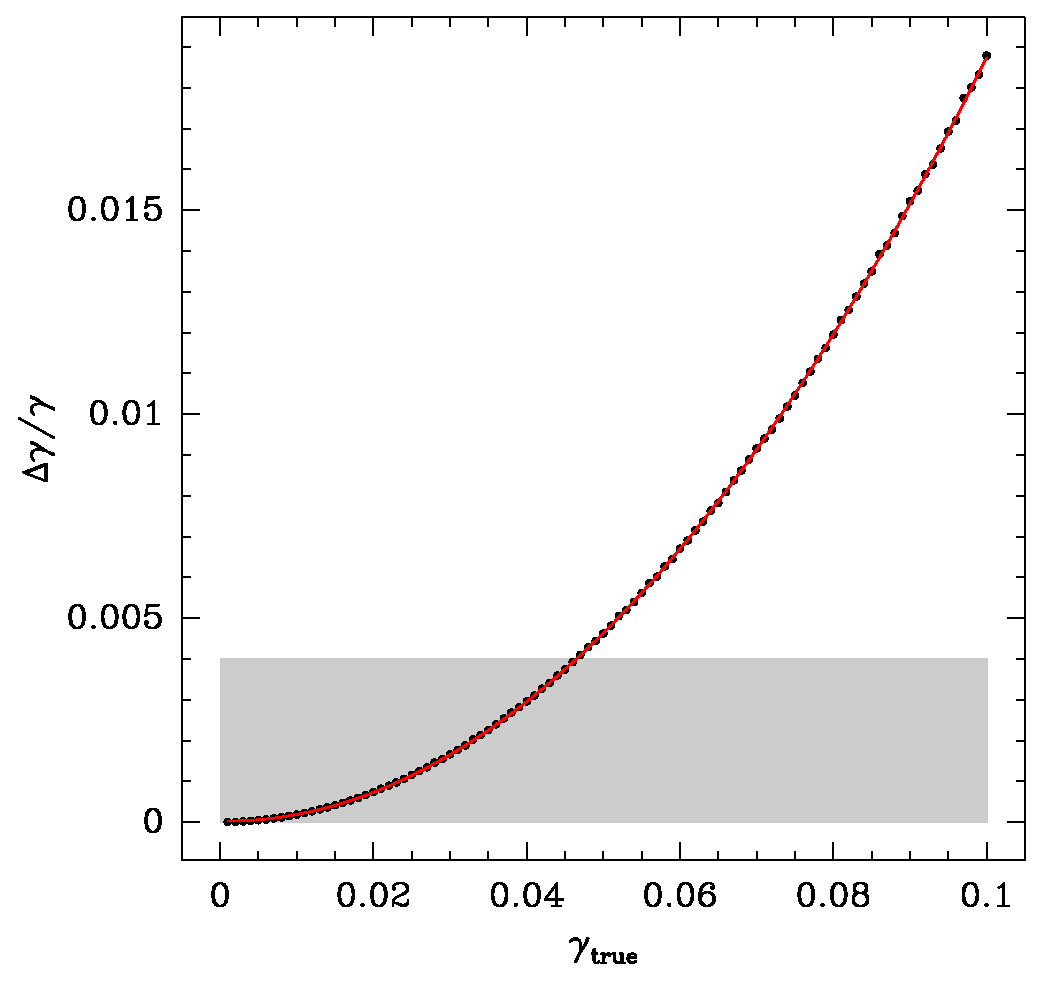
\includegraphics[scale=0.6]{figures/fracerr-vs-shear.eps}

 \caption{Fractional bias in the recovered shear $\Delta g/g = g/g_{true}-1$
     as a function of true shear,
     in a zero noise simulation.  The blue circles represent the recovered
     shear when using the posterior equations expanded to second order about
     zero shear.  The red diamonds represent expansion about the true shear.
     The solid curve represents the best-fitting quadratic function of the true
     shear $\Delta g/g \sim 1.9~g^2_{true}$.  The quadratic bias as a function of
     true shear indicates a break down of the second-order approximation
 presented in \cite{ba14}. The light and dark gray bands represent the
 requirements for current and planned surveys respectively.
 \label{fig:nonoise}}

\end{figure}

Because of this bias, I expanded the equations about the true shear rather than
zero shear, as explained in \S \ref{sec:simfit}.

\subsection{Calibration Bias vs. Galaxy \sn\ and Size} \label{sec:snbias}

Figure \ref{fig:fracerr} contains ...  \S \ref{sec:sim}, representing different
galaxy types and sizes.  TODO figure out how to split the figures up; probably
based on size, but maybe by \sersic\ index?

\begin{figure}[p] \centering
 \centering 
 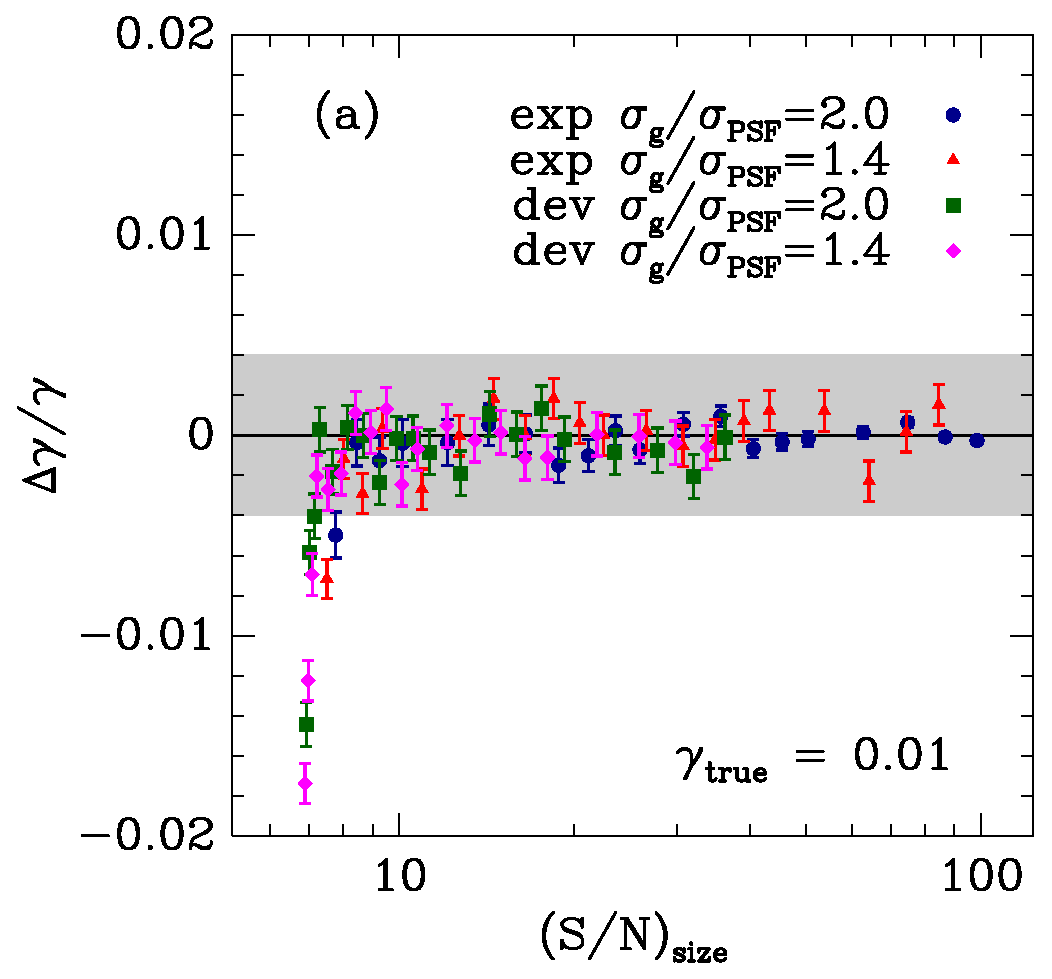
\includegraphics[scale=0.45]{figures/cbafit-geg-T-s2n.eps}
 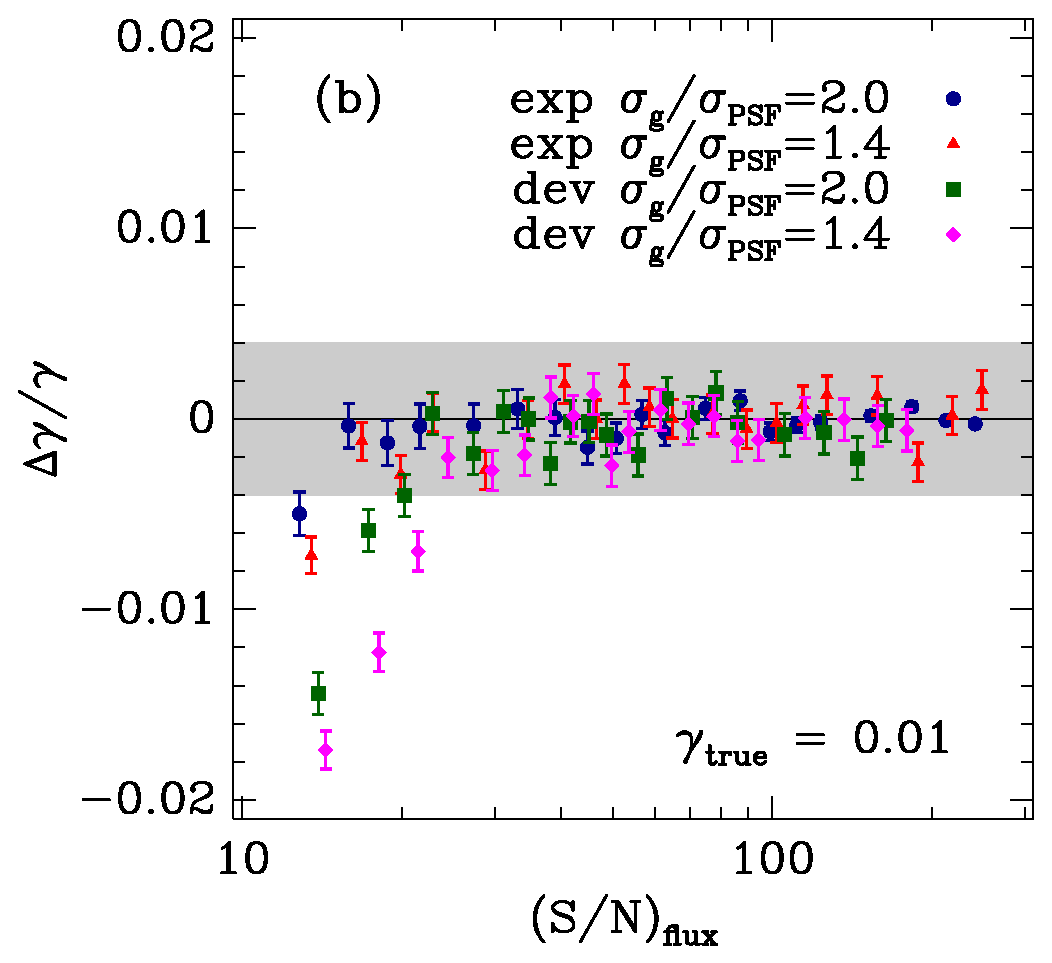
\includegraphics[scale=0.45]{figures/cbafit-geg-flux-s2n.eps}

 \caption{ Fractional bias in the recovered shear for the estimator presented
     in \cite{ba14}.  The bias is plotted as a
     function of galaxy signal-to-noise ratio \sn, for various galaxy
     properties and two different measures of \sn.  In panel (a) is
     plotted \Tsn, where the measure of intrinsic galaxy size is $T=I_{xx} + I_{yy}$.  In 
     panel (b) is plotted \fsn.  The flux and $T$ are parameters in the model
     fits, and the associated \sn\ is the ratio of best-fit value to error in
     the fit.  In each panel the fractional error is plotted for galaxies of
     different size and type, as described in the text.  As shown panel (a)
     panel, the bias depends uniquely on \Tsn\ for different galaxy types and
     sizes.  However, \fsn\ is not a sufficient descriminator for different
     galaxy types and sizes.  The \Tsn\ can be used to remove galaxies from the
     sample that will yield poor shear estimates, independent of galaxy
     properties, but not so \fsn.  For \Tsn$~ \gtrsim 10$ this shear estimator meets
 the accuracy requirements for the Dark Energy Survey, shown as the gray band.
 \label{fig:fracerr}}

\end{figure}

The fractional bias is shown as a function of signal-to-noise ratio \sn,
for two definitions of \sn, \Tsn\ and \fsn.  The traditional measure of
signal-to-noise ratio is \fsn, defined as the best fit value of total flux
divided by the error in the fit.  A more useful definition of signal-to-noise
ratio is \Tsn, the signal-to-noise ratio of the galaxy intrinsic, pre-seeing
size.  As expected, fits to noisy galaxies will result in a noisy determination
of size, and also a noisy shear measurement. But small galaxies are also more
difficult to fit, even at higher values of flux signal-to-noise ratio.  Thus it
is intuitive that small galaxies may also yield poor shear estimates.

The fractional bias in the recovered shear is, within errors, uniquely
determined by \Tsn.  But for \fsn, the fractional bias depends also on galaxy
type and size, indicating the \fsn\ is not a sufficient statistic for
determining the bias.


\subsection{Comparison with Requirements for Current and Planned Surveys}
\label{sec:req}

In the figures above I showed gray bands representing the approximate
multiplicative bias requirements for current surveys such as the Dark Energy
Survey \citep[][DES]{DESWhitePaper} and the Hyper-Suprime-Cam survey
\citep[][HSC]{HSC12}, and planned surveys such as the Large Synoptic Survey
Telescope \citep[][LSST]{IvezicLSST08} and the Euclid Mission
\citep{Euclid2011}.  These requirements are based on
\citep{HutererSystematics06} assuming fiducial sky coverage and a degredation
in the dark energy equation of state parameter of less than 20\%.  The cut at
20\% is somewhat arbitrary, and was chosen to coincide very roughly with the
``official'' requirements for DES. The requirements are $\sim$\desreq\ for
current surveys and $\sim$\lsstreq\ for planned surveys.  These requirements
are met in all the cases that I tested.

Yet I did detect some small bias in a number of cases, and the bias is
generally larger for smaller galaxies.  If this bias were related to noise I
would expect the error to be worse for low \sn\ images, but the bias is similar
at intermediate and high \sn.  This may be a sign that the implementation
itself is flawed; perhaps the exploration of the posterior using MCMC needs
further tuning.  The simulations used in this study took millions of processor
hours, so repeating the experiments to the same precision for new MCMC
parameters is a significant task.  That exploration is left to future work.

The authors of \cite{ba14} noted that small and faint galaxies, for which the
ellipticity likelihood is broad, get little weight in the average shear
relative to larger and brighter galaxies.  This is an intrinsic feature of the
estimator, no additional weighting is needed.  Thus it may be that the bias
seen for very small galaxies will not propagate significantly into measurements
performed on real data.  Yet small galaxies are more numerous than large
galaxies in a flux-limited sample, so as a whole the population of small
galaxies may indeed have weight.  It may be worth while to make cuts on galaxy
size, and in fact some cut will indirectly be made in the process of
star-galaxy selection.  But care must be taken not to introduce selection
biases. A more realistic simulation, with galaxy images that mimic a
flux-limited sample, can test this reasoning, but is beyond the scope of this
work.

In Figure \ref{fig:nonoise} I showed the multiplicative bias due to the
breakdown of the second-order taylor expansion at higher shear.   This effect
is prohibitive for current surveys when the shear exceeds 0.05.  An
implementation using higher order information, a different expansion, or
perhaps a full mapping of the posterior of the shear will be required to
recover larger shears to sufficient accuracy.  Simply correcting the result
based on the curve in figure \ref{fig:nonoise} might be sufficient (TODO test
that).

\section{Summary} \label{sec:summary}

TODO merge these paragraphs some how.

I used a model fitting approach in this work, but true galaxies cannot be fully
described by a finite number of parameters.  \cite{Kacprzak13} show that this
``model bias'' may be on the order of baseline requirements for current
surveys, but potentially crippling for future surveys with more stringent
requirements. One potential solution is to fit models with more freedom, but
this will be accompanied by relatively larger noise in the recovered shear.
\cite{ba14} propose an alternative to the model-fitting technique based on
moments in Fourier space which makes no explicit parameterization of galaxy
light distributions.  An evaluation of this model free approach in the presence
of noise is worthy of study.

This model-fitting approach is useful as a proof-of-principle:  model-fitting
is limited by the accuracy of the models to represent true galaxies, and thus
in real data additional errors be present.  But if the shear can be recovered
in a controlled simulation, fitting known models, this is a strong
encouragement for further development of this method.


\section*{Acknowledgments}

ES is supported by DOE grant DE-AC02-98CH10886.

Thanks to Gary Bernstein, Bob Armstrong, and Anze Slosar for many useful
discussions; thanks to Anze for suggesting I expand the equations about the
true shear to reduce the number of simulated images required for each test.
Thanks to the STAR, PHENIX and LBNE experiments at BNL for use of spare cycles
on their compute clusters, and to the RACF staff at BNL for their continued, and
disproportionately large support of my work.


\bibliographystyle{apj}
% Bib database
\bibliography{apj-jour,astroref}

\end{document}

